\section{溶解的过程}\label{sec:4-2}

物质是怎样溶解到水里的?在溶解的过程中发生了什么变化?
我们把蔗糖溶解于水,作为一个例子,来说明物质是怎样溶解到水里的。

把蔗糖放在水里,蔗糖表面的分子在水分子的作用下,克服了蔗糖分子之间的引力,
有的分子就脱离了蔗糖的表面,在水里扩散。
可见,蔗糖的溶解过程是蔗糖分子在水分子的作用下,向水里扩散的过程。

为了进一步研究物质在溶解过程中所发生的变化,我们先观察下面实验里的现象。

\begin{figure}[htbp]
    \centering
    \begin{minipage}[b]{7cm}
        \centering
        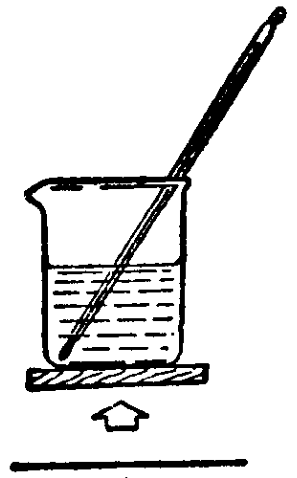
\includegraphics[width=4cm]{../pic/czhx1-ch4-1-1}
        \caption*{I. 硝酸铵溶于水}
    \end{minipage}
    \qquad
    \begin{minipage}[b]{7cm}
        \centering
        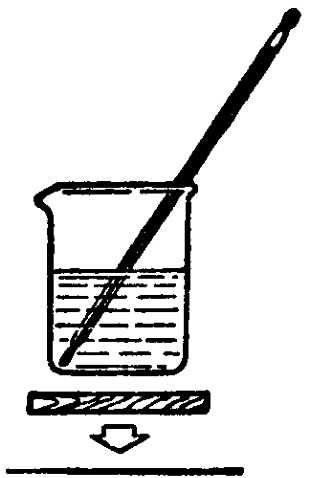
\includegraphics[width=4cm]{../pic/czhx1-ch4-1-2}
        \caption*{II. 浓硫酸溶于水}
    \end{minipage}
    \caption{溶解的吸热现象和放热现象}\label{fig:4-1}
\end{figure}

\begin{shiyan}
    按图 \ref{fig:4-1} I 把一个小烧杯放在一块刨光的小木板上,木板上先加一些水。
    然后在烧杯里注入 100 毫升水,把温度计放入烧杯里,再加入 50 克硝酸铵(\ce{NH4NO3}),
    小心地用温度计搅动溶液(防止把温度计碰坏,并注意温度的变化),观察有什么现象发生。
\end{shiyan}


硝酸铵溶于水,溶液的温度显著降低,使烧杯和木板之间的水结成薄冰,拿起烧杯时,可以看到,
和烧杯底冻结在一起的木板也同时被提起。这充分说明,硝酸铵溶解于水时要吸收热量。

\begin{shiyan}
    按图 \ref{fig:4-1} II 把一个小烧杯用熔化的蜡粘结在一块小木扳上,然后在烧杯里加入 100 毫升水,
    再注入 40 毫升浓硫酸(注意要慢慢地注入),边注入,边用温度计小心地搅动,观察有什么现象发生。
\end{shiyan}

浓硫酸溶于水,溶液的温度显著升高,溶解时放出大量的热,使烧杯下的蜡熔化,
拿起烧杯时,木板就掉下来。这充分说明,浓硫酸溶解于水时要放出热量。

怎样解释物质溶解时,有的吸热,而有的放热呢?

这是因为,物质溶解在水里,通常发生两种过程:
一种是溶质的分子(或离子)的扩散过程,这种过程吸收热量,是物理过程;
另一种是溶质的分子(或离子)和水分子作用,形成水合分子(或水合离子)的过程,这种过程放出热量,是化学过程。

物质溶解的时候,溶液的温度是升高还是降低,要看在这两种过程里,
是放出的热量多于吸收的热量,还是吸收的热量多于放出的热量而定。
例如,硝酸铵溶解在水里的时候,吸收的热量多于放出的热量,所以溶液的温度降低。
相反,硫酸  溶解在水里的时候,放出的热量多于吸收的热量,所以溶液的温度升高。

由此可见,溶解过程中既包括物理过程,又包括化学过程。
溶液是由溶剂的分子、溶质的分子(或离子)和它们相互作用的生成物(水合分子或水合离子)等物质所组成。


\begin{xiti}

    \xiaoti{有人说:“硝酸铵溶于水吸热,只有溶质的扩散过程;
        而浓硫酸溶于水放热,只有溶质的水合过程” 。你认为对吗?为什么?
    }

    \xiaoti{溶液跟机械的混和物有什么不同?举例说明。}

\end{xiti}


